\documentclass[tikz, border=15pt]{standalone}
\usepackage[utf8]{inputenc}
\usepackage[T5]{fontenc}
\usepackage{lmodern}
\usepackage{xcolor}
\usepackage{graphicx}
\usetikzlibrary{positioning, calc, arrows}

\begin{document}
\begin{tikzpicture}[
  >=stealth,
  font=\sffamily,
  dashedContainer/.style={
    draw=black,
    dashed,
    line width=1.2pt,
    fill=white,
    rounded corners=6pt,
    inner sep=8pt,
    align=center
  },
  arrowThick/.style={
    ->,
    line width=1.8pt,
    draw=black
  },
  tagText/.style={
    font=\small\bfseries,
    fill=white,
    inner sep=3.5pt,
    rounded corners=2pt,
    draw=gray!30,
    line width=0.5pt,
    text=black
  }
]

% 1. BÊN TRÁI: BÀN TAY MANG NẸP
\node[dashedContainer, text width=5.6cm, minimum height=6.5cm] (hand_box) at (-8.5, 0) {
  {\bfseries\large BÀN TAY MANG NẸP}\\[6pt]
  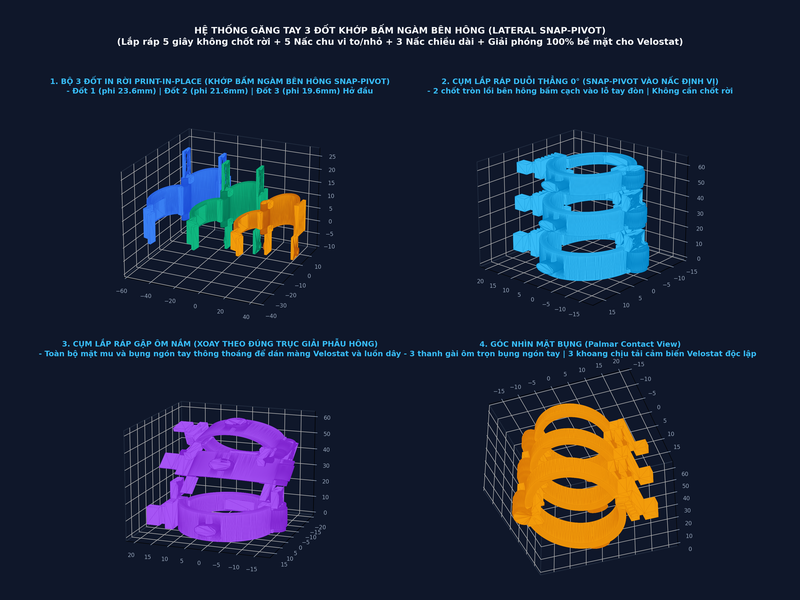
\includegraphics[width=5.0cm, height=3.6cm, keepaspectratio]{assets/splint_3d.png}\\[6pt]
  {\bfseries\normalsize Khung nẹp 3 ngón in 3D}\\[2pt]
  {\footnotesize 16 Ô Velostat vi sai + 3 Cảm biến Flex}
};

% 2. TRÊN CÙNG Ở GIỮA: CAMERA RGB & DEPTH ANYTHING V2
\node[dashedContainer, text width=7.2cm, minimum height=4.2cm] (vis_box) at (0, 3.6) {
  {\bfseries\large THỊ GIÁC ĐÓN TRƯỚC}\\[4pt]
  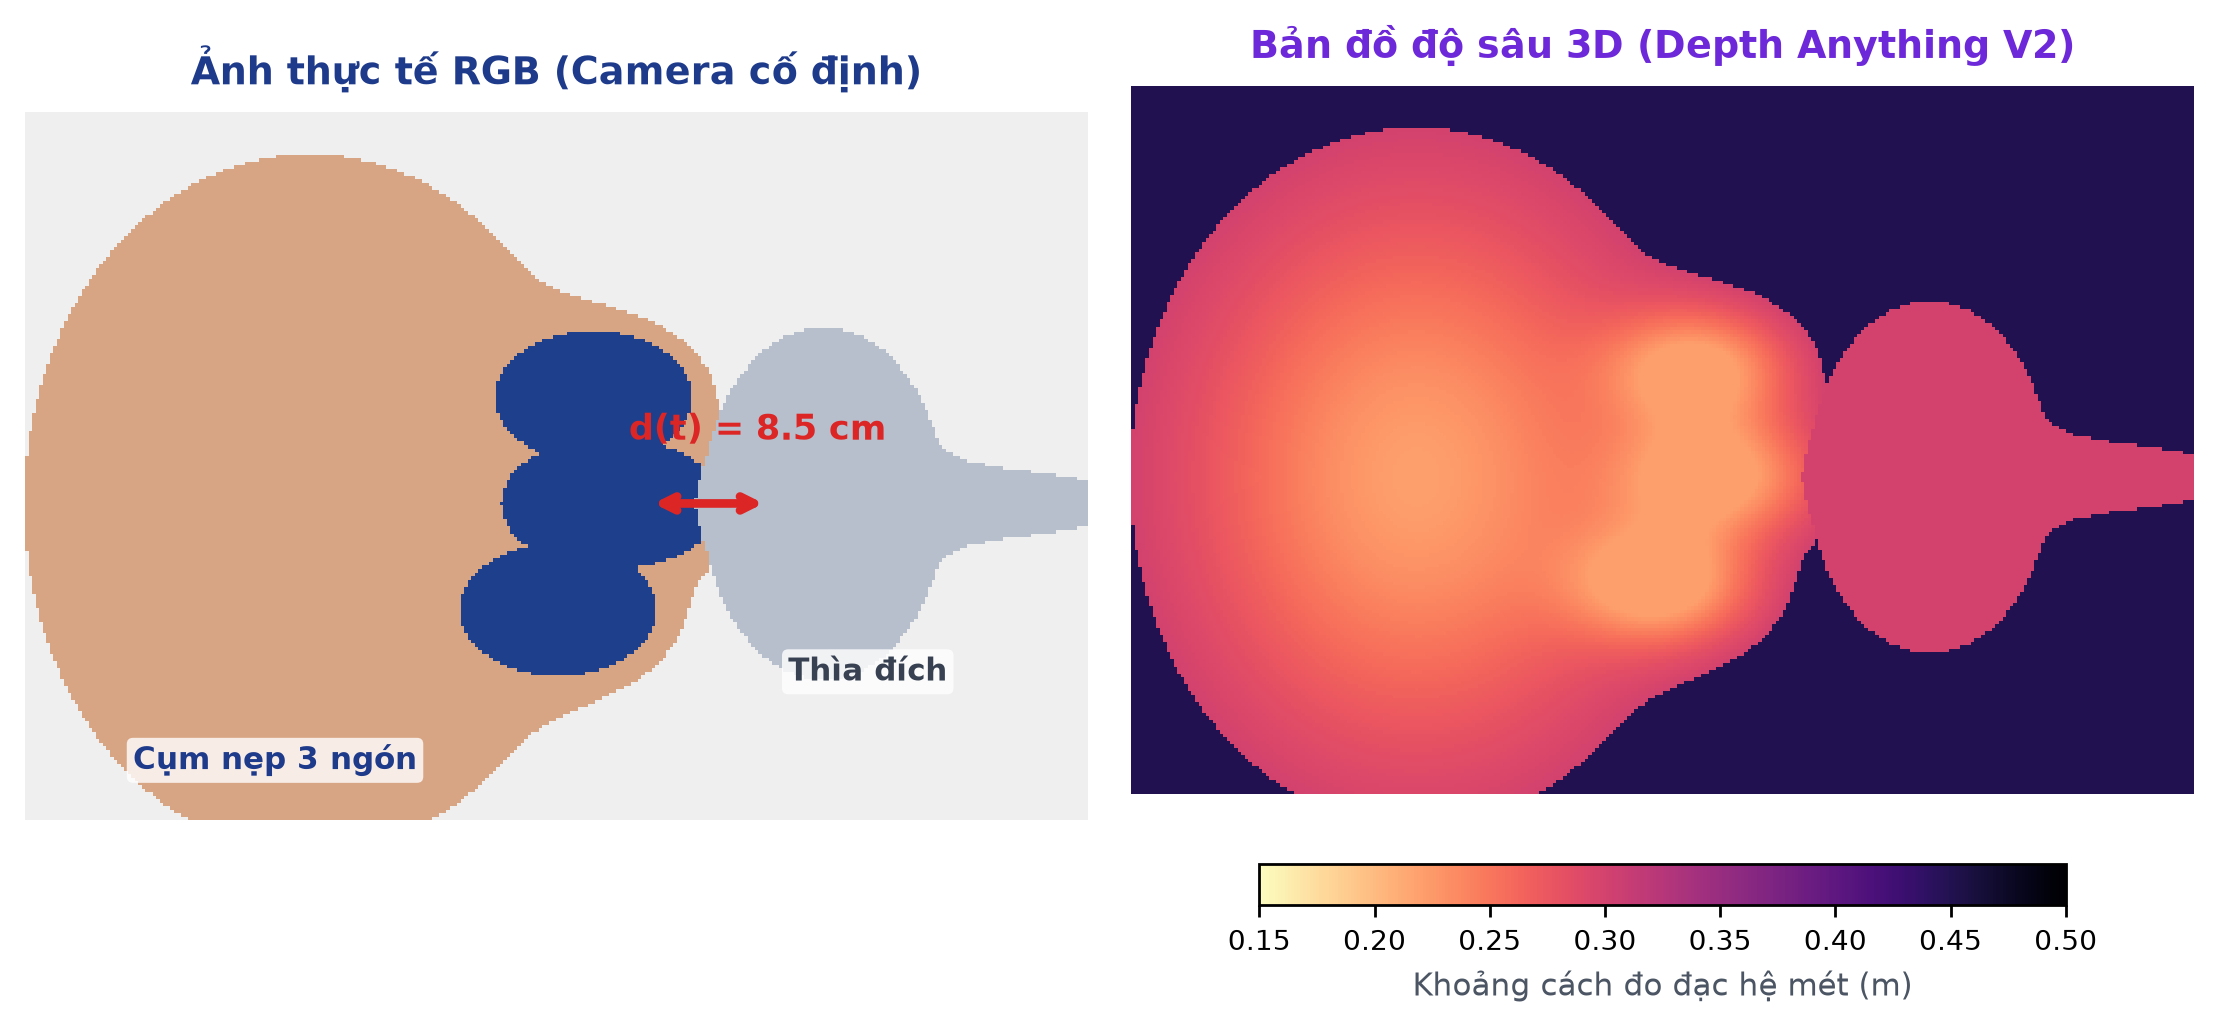
\includegraphics[width=6.8cm, height=2.6cm, keepaspectratio]{assets/depth_anything_scene.png}\\[4pt]
  {\bfseries\small Camera RGB + Depth Anything V2 (3D)}\\[2pt]
  {\footnotesize Ước lượng cự ly $d(t)$ \& Thời gian tới tiếp xúc (TTC)}
};

% 3. BÊN PHẢI: BỘ ĐIỀU KHIỂN ESP32-S3 + ADS1115
\node[dashedContainer, text width=6.2cm, minimum height=6.5cm] (ctrl_box) at (8.5, 0) {
  {\bfseries\large BỘ ĐIỀU KHIỂN TRUNG TÂM}\\[6pt]
  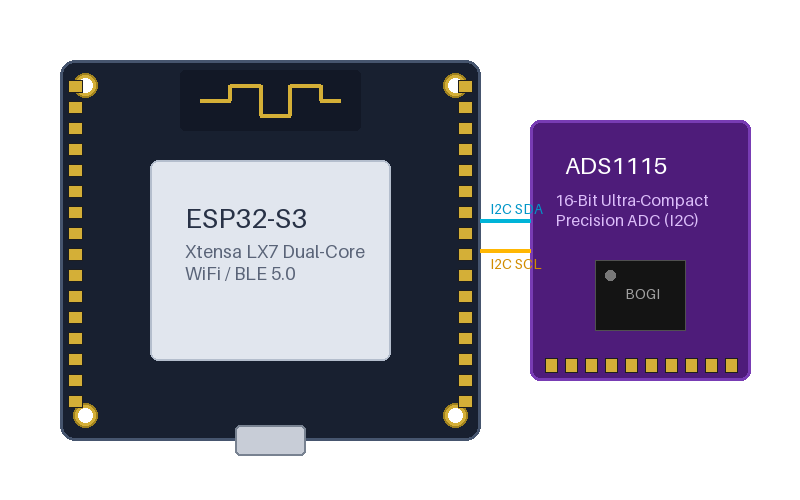
\includegraphics[width=5.4cm, height=3.0cm, keepaspectratio]{assets/controller_ads_board.png}\\[6pt]
  {\bfseries\normalsize ESP32-S3 + ADC ADS1115}\\[2pt]
  {\footnotesize Lọc số DSP 2 nhánh $\bullet$ Tính toán EI -- GAP -- RAL\\[2pt]
  Thuật toán trợ lực theo nhu cầu (AAN 3 pha)}
};

% 4. DƯỚI CÙNG Ở GIỮA: TRỢ LỰC SERVO & TANG CÁP
\node[dashedContainer, text width=7.2cm, minimum height=4.2cm] (act_box) at (0, -3.6) {
  {\bfseries\large CƠ CẤU TRỢ LỰC CƠ HỌC}\\[4pt]
  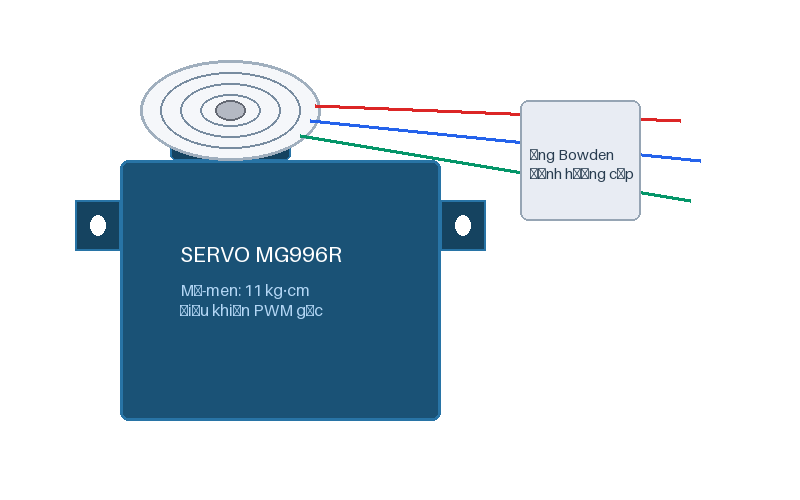
\includegraphics[width=6.6cm, height=2.6cm, keepaspectratio]{assets/servo_spool_assembly.png}\\[4pt]
  {\bfseries\small 3 Động cơ Servo MG996R \& Tang cuốn cáp}\\[2pt]
  {\footnotesize Truyền động cáp Bowden kéo gập / Nhả duỗi ngón tay}
};

% ==================== MŨI TÊN VÒNG LẶP KHÉP KÍN TO RÕ (LANDSCAPE) ====================

% Từ Tay -> Camera (Quan sát)
\draw[arrowThick] (hand_box.north) |- node[tagText, near end, above=2pt] {Quan sát cự ly 3D tay -- thìa} (vis_box.west);

% Từ Camera -> ESP32-S3 (Khẩu độ \& TTC đón trước)
\draw[arrowThick] (vis_box.east) -| node[tagText, near start, above=2pt] {Khẩu độ \& TTC đón trước} (ctrl_box.north);

% Từ Tay -> ESP32-S3 (Tín hiệu lực và góc gập)
\draw[arrowThick] (hand_box.east) -- node[tagText, above=2pt] {Tín hiệu cảm biến (Lực tiếp xúc \& Góc gập)} (ctrl_box.west);

% Từ ESP32-S3 -> Servo (Lệnh điều khiển servo AAN)
\draw[arrowThick] (ctrl_box.south) |- node[tagText, near end, below=2pt] {Lệnh servo AAN} (act_box.east);

% Từ Servo -> Tay (Vòng cơ học kéo gập / nhả duỗi)
\draw[arrowThick] (act_box.west) -| node[tagText, near start, below=2pt] {Cáp Bowden trợ lực kéo gập / Nhả duỗi mở ngón} (hand_box.south);

\end{tikzpicture}
\end{document}
